Hier soll etwas stehen

\chapter{Strategie}
Um die Ausgangslage zu verbessern können verschiedene Ansätzte gewählt werden. In diesem Konzept wird vorallem

\section{Ziel}
Sollte ein bestimmtes Exemplar verloren gehen, soll diese automatisiert im Hochregallager wiedergefunden werden.

\section{Wirkung}
Die so vereinfachte Wiederfindung soll der Speicherbibliothek zu einer erhöhten Sicherheit bezüglich der Einlagerung der Exemplare verhelfen. Es soll bewirkt werden, dass deplatzierte Exemplare ohne grösseren personellen Aufwand wiederbeschafft werden können.

\section{Zielgruppe}
Die direkte Zielgruppe ist die Speicherbibliothek selbst. Diese könnte somit der indirekten Zielgruppe eine noch höhere Garantie gewährleisten.

Die Indirekte Zielgruppe währen demnach alle der Speicherbibliothek angeschlossenen Bibliotheken, sowie deren Kunden, welche Seiten bestimmter Exemplare als eingescannte Datei bestellen oder ausgewählte Exemplare mit einer Voranmeldung vor Ort lesen wollen.

\chapter{Ideenbeschreibung}


Momentan fährt der Roboter nur die im System hinterlegte Position des Behälters an. Diese Fahrt wird durch die Software des Logistiksystems mitsamt des Roboters gesteuert. Neu soll die Software dieses Herstellers so erweitert werden (Siehe \ref{sec:roboterSWAnpassung}), dass der Roboter einen vordefinierten Pfad abfährt mit einem speziellen RFID Lesebehälter/Suchbehälter (Siehe \ref{sec:behaelterMitRFID}) und dabei noch Aktionen ausführt, wie die temporäre Einlagerung dieses Behälters und Zwischenlagerung des Behälters welcher sich an der eingelagerten Stelle befand.
Würde nun ein Buch, welches von einer Bibliothek oder einem anderen Kunden bestellt wurde, nicht im entsprechenden Behälter zu finden sein, soll neu der spezielle RFID Lese-/Suchbehälter in das Hochregallager geschickt werden.


Dabei gibt es zwei Unterschiedliche Suchmodi. Als Erstes würde der Roboter mit dem Lese-/Suchbehälter in alle Gassen geschickt, wo dieser durch jede Reihe nacheinander fährt. Dabei wird jeweils vom Lese-/Suchbehälter der Vordere Behälter nach dem fehlenden Exemplar abgesucht. So kann in einer Kurzer Zeit ca. 50\% des Lagers nach dem deplatzierten Exemplar abgesucht werden. Würde nach diesem Suchvorgang die Lokalisation des Exemplares nicht erfolgreich abgeschlossen werden, würde in der Nacht die zweite Suchfunktion starten, bei welcher der Lese-/Suchbehälter im Hochregallager in der Höhe jeden dritten Platz eines äusseren bereits abgesuchten Behälters für eine kurze Zeit tauscht. Während der Lese-/Suchbehälter am äusseren Platz ist sucht er im hinteren Behälter nach dem Exemplar sowie in den dem abgesuchten Behälter direkt Benachbarten Behältern.

\section{Anpassungen Lagerverwaltungssoftware}
\label{sec:roboterSWAnpassung}
Für die Software der Lagerverwaltung soll die Herstellerfirma dieser Software diese um eine Schnittelle erweitern, welche es ermöglicht dem Roboter über das Netzwerk neue Fahrpositionsdaten mitzuteilen, zu welchen er anschliessend fährt. Es soll dabei möglich sein dem Roboter zu sagen, ob er einen Behälter tauschen soll oder nur an die Position fahren soll. Zudem soll die momentane Position des Roboters über diese Schnittelle abgefragt werden können. 

\section{Behälter mit RFID Ausrüstung}
\label{sec:behaelterMitRFID}
Die heutige RFID HF Technologie, welche bereits in der Speicherbibliothek zum Einsatz kommt ist auf ca. 1m Distanz beschränkt. Dies bedeutet, dass es nicht möglich ist alle Tags direkt vom Roboter aus zu lesen. Um alle Behälter auslesen zu können muss also der Behälter die Position eines anderen Behälters einnehmen, um den hinteren Behälter lesen zu können. Da es jedoch enorm zeitintensiv ist, jede vordere Kiste mit dem Lese-/Suchbehälter auszutauschen, sollen multiple Antennen zum Einsatzt kommen. Diese sollen so ausgerichtet werden, dass nicht nur der hintere Behälter sondern auch dessen Nachbarn ausgelesen werden können.
Die Antennen sollen gemäss Abbildung \ref{fig:antennenPositionen} ausgerichtet werden.

\begin{figure}
	\centering
	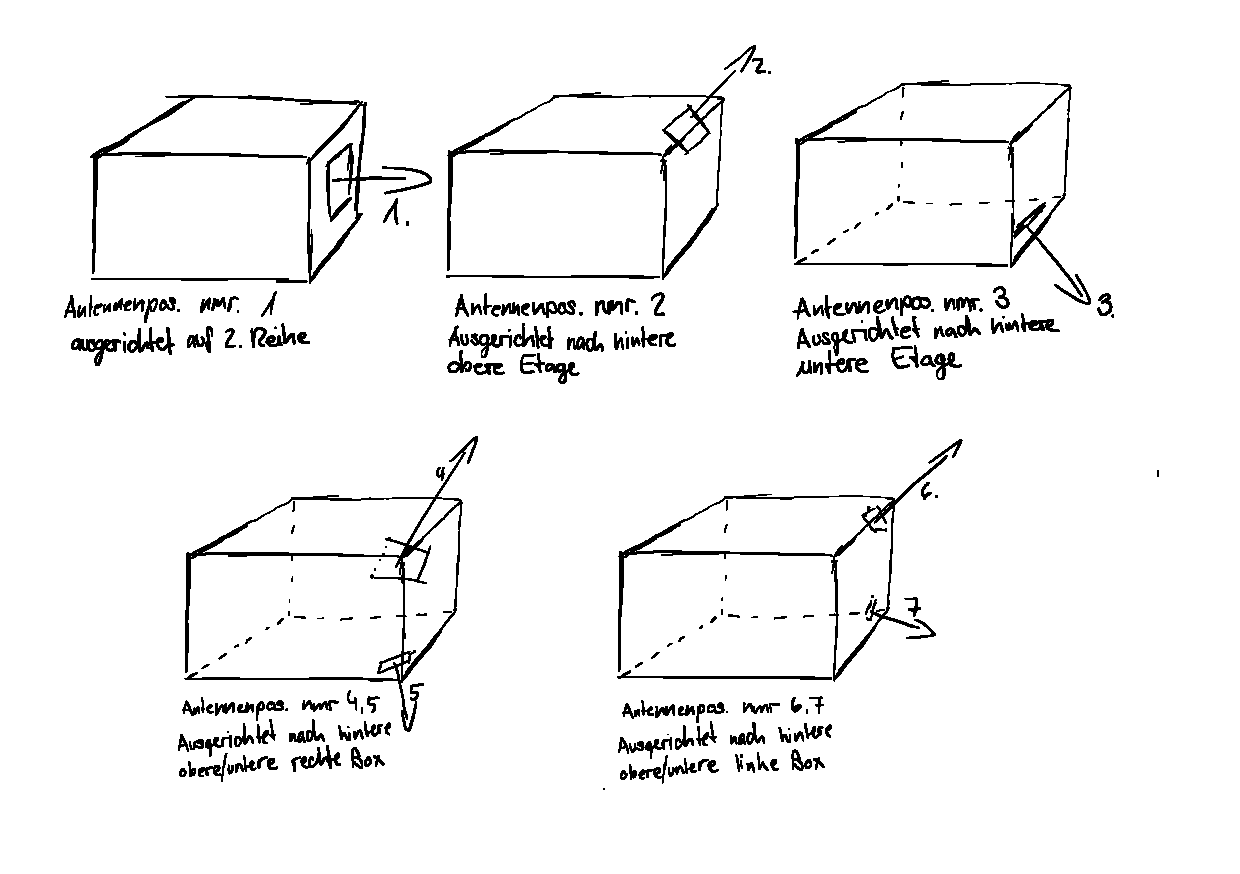
\includegraphics[keepaspectratio, width=1\textwidth]{antennen_auf_behaelter}
	\caption{Alle Antennenpositionen in einer Box für die Rechte Seite}
	\label{fig:antennenPositionen}
\end{figure}

In der Abbildung \ref{fig:distanzcalc} wird dargestellt, dass alle äussere Behälter noch innerhalb der von HF RFID möglichen Lesedistanz von unter 1m liegen.

\begin{figure}
	\centering
	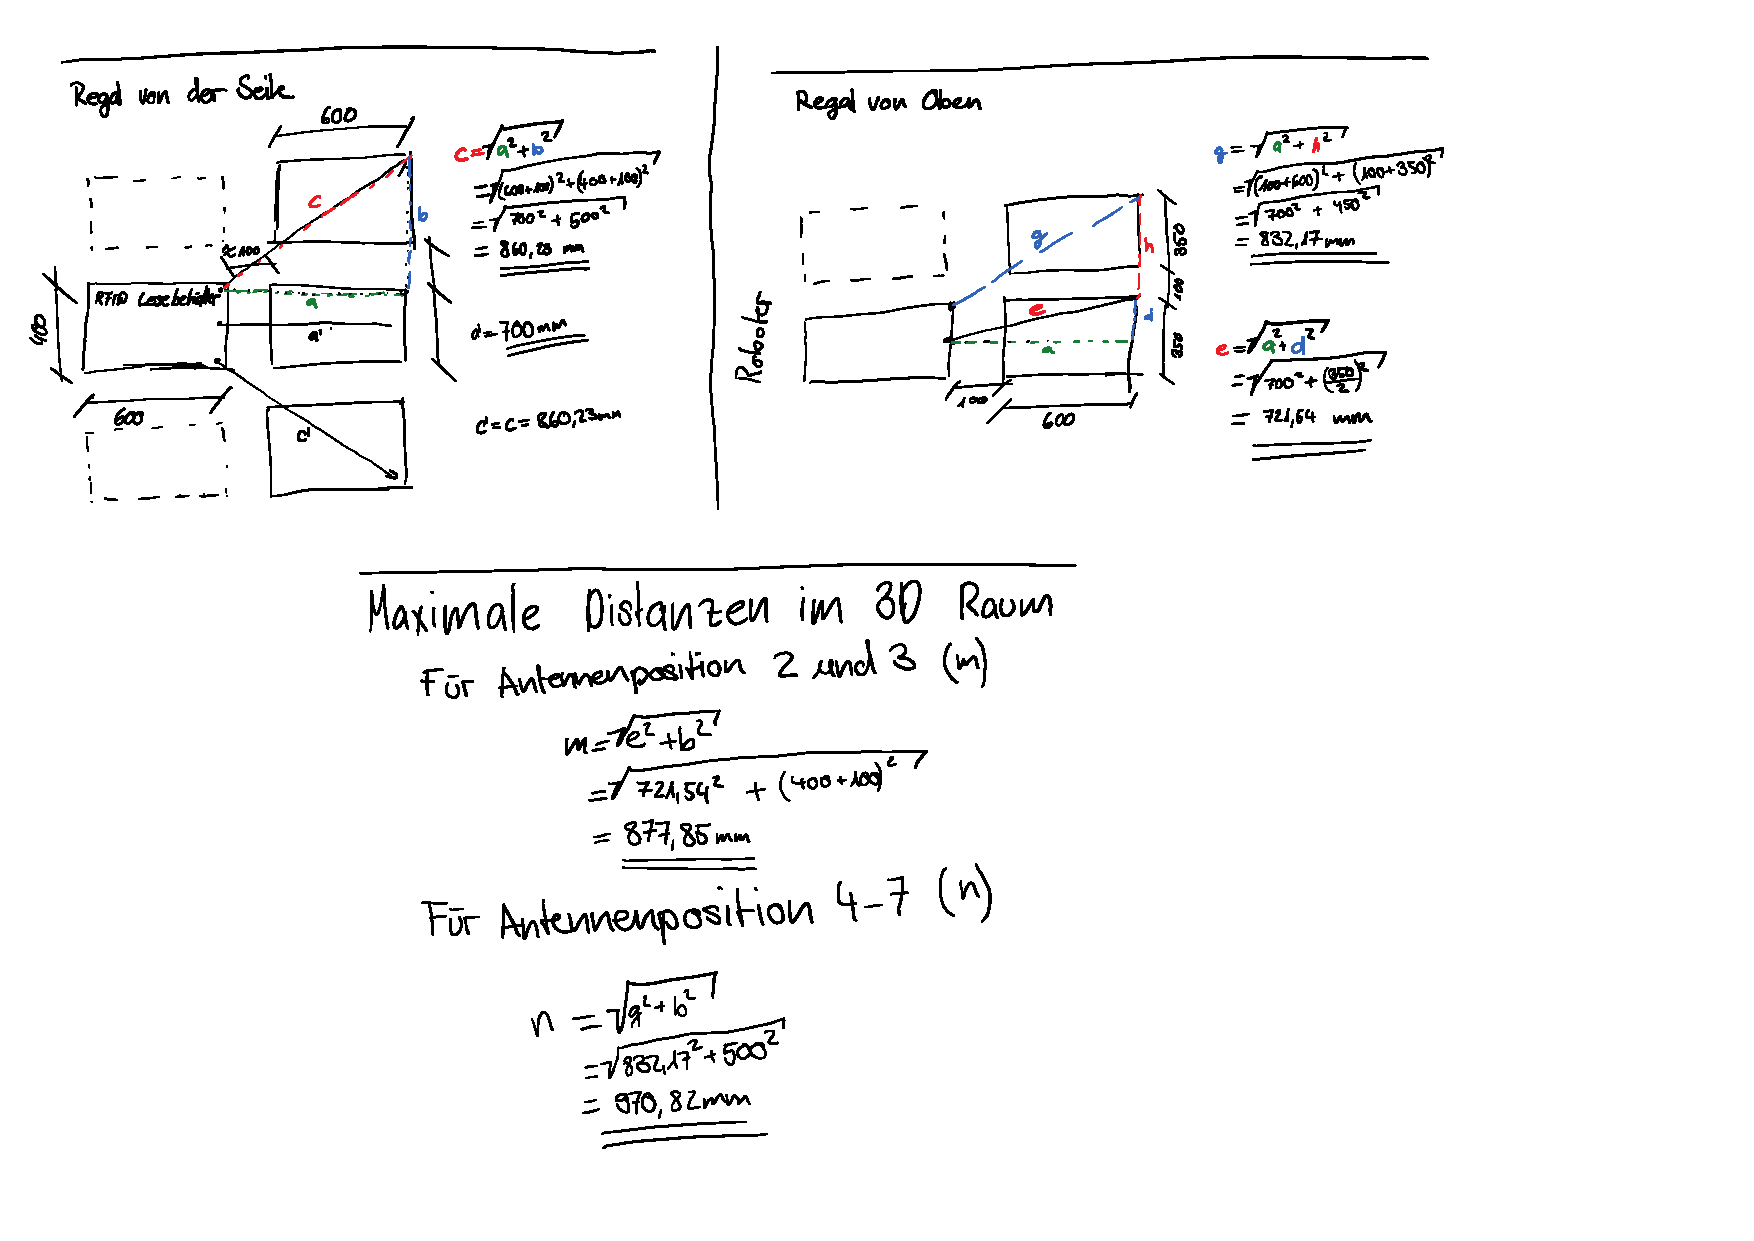
\includegraphics[keepaspectratio, width=1.2\textwidth]{berechnung_maximaler_distanz}
	\caption{Berechnung der maximalen Distanzen (alle Angaben in mm)}
	\label{fig:distanzcalc}
\end{figure}

\chapter{Zeitplan}

\chapter{Finanzierungsplan}

\chapter{Dokumentation und Evaluation}